\documentclass[12pt]{article}
\usepackage{fontspec}
\usepackage[utf8]{inputenc}
\setmainfont{Bodoni 72 Book}
\usepackage[paperwidth=17in,paperheight=11in,margin=1in,headheight=0.0in,footskip=0.5in,includehead,includefoot,portrait]{geometry}
\usepackage[absolute]{textpos}
\TPGrid[0.5in, 0.25in]{23}{24}
\parindent=0pt
\parskip=12pt
\usepackage{nopageno}
\usepackage{graphicx}
\graphicspath{ {./images/} }
\usepackage{amsmath}
\usepackage{hyperref}
\usepackage{tikz}
\newcommand*\circled[1]{\tikz[baseline=(char.base)]{
            \node[shape=circle,draw,inner sep=1pt] (char) {#1};}}

\begin{document}

\begingroup
\begin{center}
\huge HINWEISE FÜR DEN INTERPRETEN
\end{center}
\endgroup

\begingroup
\textbf{Allgemein: \circled{1} Vorzeichen} werden für jeden Takt gesetzt, aber sie werden nochmal gesetzt, wenn die gleiche Note später im selben Takt auftritt - außer die Note wird unmittelbar wiederholt. \textbf{\circled{2}} Die in Anführungszeichen gesetzte \textbf{Dynamik} bezieht sich nicht auf die Lautstärke des Klangs, sondern auf den Druck der Werkzeuge. \textbf{\circled{3}} Wenn eine \textbf{Linie von einer Note ausgeht} und sich nach unten zu einer anderen Note neigt, wie unten: 

\begin{center}
\includegraphics[scale=0.45]{interruptive_polyphony.png}
\end{center}

Dem Interpreten sollte die \textbf{Dauer der aktuellen Note} zu Beginn einer nachfolgenden Note in einer parallelen Stimme \textbf{verkürzen} und so weit wie möglich versuchen, die Unabhängigkeit der einzelnen Linien zu verdeutlichen. Dies wird durch diagonale Linien kontrastiert, die von Note zu Note gezogen werden, wie unten dargestellt: 

\begin{center}
\includegraphics[scale=0.40]{hocket.png}
\end{center}

die lediglich als \textbf{Hilfsindikatoren} für die \textbf{Notenssequenzierung} über die Notensysteme hinweg bei komplexen Polyrhythmen dienen. \textbf{\circled{4} Flache Glissandi } werden in ähnlicher Weise wie Bindebögen verwendet, aber während Bindebögen auf die Darstellung metrischer Pulsgruppierungen während einer einzelnen Note beschränkt sind, binden flache Glissandi komponierte Rhythmen, um als \textbf{Ankernoten für dynamische Veränderungen} innerhalb einer anhaltenden einzelnen Note verwendet zu werden. \textbf{\circled{5}} Die Partitur folgt dem Notationsbeispiel von Luigi Nono, der die vertraute, gewölbte \textbf{Fermate} als Orientierungspunkt verwendete. Den Bogen zu \textbf{triangulieren} bedeutet, die Fermate zu \textbf{verkürzen}, und den Bogen zu \textbf{quadrieren}, bedeutet, die Fermate zu \textbf{verlängern}. Die \textbf{Hinzufügung zusätzlicher Bögen} erhöht die relative Länge oder Kürze der Fermate. Dem Interpreten wird davon abgeraten, die Quantisierung zu vermeiden, indem er sein eigenes System zum Zählen der Fermaten entwickelt. Stattdessen sollten die Fermaten als Einladung verstanden werden, eher zu warten als zu zählen, wobei die Form ihrer Bögen ein Zeichen für den relativen Raum dieser Einladung ist. \textbf{\circled{6}} In dieser Partitur erhalten einige Takte eine \textbf{Taktart mit einem Nenner, der kein Exponent von 2 ist}. In jedem Fall wird das Prinzip beibehalten, das für die \textbf{Ableitung von konventionelleren Metren} ( verstanden als Unterteilungen einer ganzen Note ) gilt. Zum Beispiel bedeutet \textbf{2/10} einen Takt der aus \textbf{zwei Schlägen} besteht, von denen jeder einem \textbf{Zehntel einer ganzen Note} entspricht. Wie in vielen zeitgenössischen Musiken, in denen die Taktarten zusammengesetzter Metren den Inhalt ihrer Takte \textbf{nicht verändern} ( z. B. ist eine Viertelnote in \textbf{6/8} und in \textbf{3/4} immer gleich schnell ), wird auch bei diesen ungewöhnlichen Taktarten das Tempo beibehalten. \textbf{\circled{7} Tuplet-Klammern, die nicht auf einer Seite gebogen sind}, wie unten:

\begin{center}
\includegraphics[scale=0.50]{ungewöhnlichen_taktarten.png}
\end{center}

geben die \textbf{Prolation} ( ,,Prolation", aus dem Englischen entlehnt, bedeutet die ,,rationale Umproportionierung" eines Tempos ) einer Note allein an, ohne die Anzahl der Noten innerhalb der Prolation anzugeben. \textbf{\circled{8}} Obwohl die Verwendung des \textbf{Haltepedals} an mehreren Stellen in der Partitur ausdrücklich vorgeschrieben ist, schließt dies \textbf{nicht} den Ermessensspielraum der Interpreten an Stellen aus, an denen die Verwendung des Haltepedals nicht ausdrücklich vorgeschrieben ist.
\endgroup

\begingroup
\textbf{Bühne: \circled{1}} Diese Partitur wird mit einem \textbf{undurchsichtigen Vorhang} aufgeführt, der den Pianisten und die Zuhörer \textbf{trennt}. Die beiden Lautsprecher, die für die unter ,,\textbf{Elektronik}" erläuterte Verstärkung verwendet werden, sind \textbf{vor} dem Vorhang platziert und für die Zuhörer \textbf{sichtbar}.
\endgroup

\begingroup
\textbf{Elektronik: \circled{1}} In diesem Stück wird das \textbf{Zuspiel} ( beim Komponist erhältlich ) nur in den \textbf{ersten 6 Takten verwendet}. Es wird empfohlen, dass dem Interpreten und nicht ein Techniker den Anfang des Zuspiels kontrolliert, um die Anpassung des Tempos zu erleichtern. \textbf{\circled{2}} Das Klavier wird von \textbf{zwei Lautsprechern verstärkt}, um ein Stereobild zu erzeugen (tiefe Tasten = links, hohe Tasten = rechts), vor allem um die durch den Vorhang verursachte Schalldämpfung zu verdeutlichen. \textbf{\circled{3}} Das zu verstärkende Signal sollte auch durch einen \textbf{Tiefpassfilter} laufen, der vom Interpreten über ein \textbf{Fußpedal} gesteuert wird. Dieses Fußpedals wird mit \textbf{Linien auf einem zweizeiligem Notensystem} komponiert, wobei die \textbf{oberste Zeile} ein vollständig \textbf{unbetätigtes Pedal}, die \textbf{unterste} ein vollständig \textbf{betätigtes} Pedal und der \textbf{Zwischenraum} eine \textbf{ungefähre Position} zwischen den beiden darstellt. \textbf{\circled{4}} Es gibt Momente in diesem Stück, in denen ein vom Komponist in Supercollider geschriebener \textbf{Synthesizer} die Signale des Klaviers verarbeitet. Dieser Synthesizer verhält sich \textbf{automatisch} und muss nur gemäß den Anweisungen in der Partitur ein- und ausgeschaltet werden. Diese Umschaltung kann vom \textbf{Interpreten} oder einem \textbf{Techniker} vorgenommen werden.
\endgroup

\begingroup
\textbf{Präparierung: \circled{1}} Das Klavier ist mit \textbf{Magneten} an drei Stellen präpariert, die erste befindet sich zwischen den Stimmwirbeln der \textbf{hohen} Saiten und den Saiten selbst, die zweite zwischen den Stimmwirbeln der \textbf{tiefen} Saiten und den Saiten selbst, und an der dritten Stelle sind 4-5 Magnete \textbf{auf  die Stimmwirbel} verteilt, wie unten dargestellt:

\begin{center}
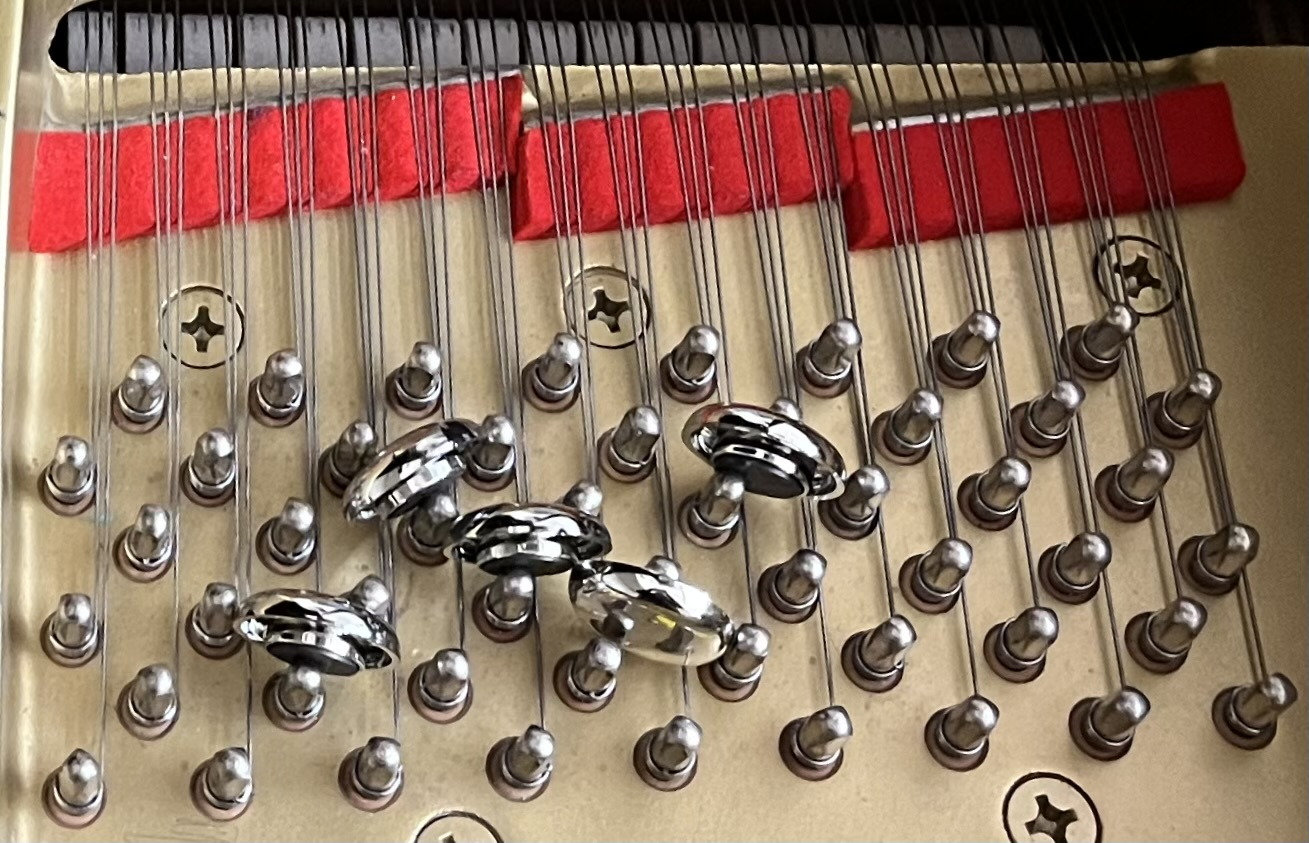
\includegraphics[scale=0.70]{magnets.jpg}
\end{center}

\textbf{\circled{2}} Gelegentlich wird ein ,,\textbf{feaux-Glissando}" erzeugt, indem man einen \textbf{Hartplastikvibrator} auf den Kopf einer \textbf{Schraube} oder eines dicken \textbf{Nagels} setzt, der \textbf{zwischen einer der Saiten} angebracht ist. Bewegt man den Nagel in \textbf{Richtung des Interpreten}, \textbf{erhöht} die Tonhöhe, \textbf{entfernt man sich vom Interpreten}, \textbf{sinkt} die Tonhöhe. Dem Interpreten wird aufgefordert, den Nagel zwischen den Saiten zu platzieren, die am bequemsten die komponierten Tonhöhen erzeugen, die je nach Instrument variieren können. \textbf{\circled{3} Eine Maultrommel} wird zwischen die Saite \textbf{D, gelegt}, so dass sich die Hälfte der Basis unter der Saite befindet. Beim Spielen des Vibrators wird eine von \textbf{drei Positionen} ( zwischen denen interpoliert werden kann ) verwendet. Diese Positionen werden im Folgenden anhand der entsprechenden Grafiken dargestellt:

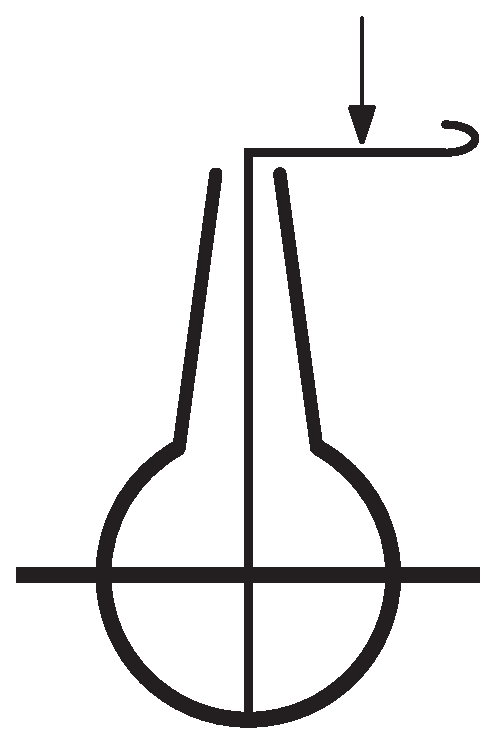
\includegraphics[scale=0.17]{crook.eps}
\circled{1} Berühren des Vibrators \textbf{an den Bogen} der Maultrommel \\

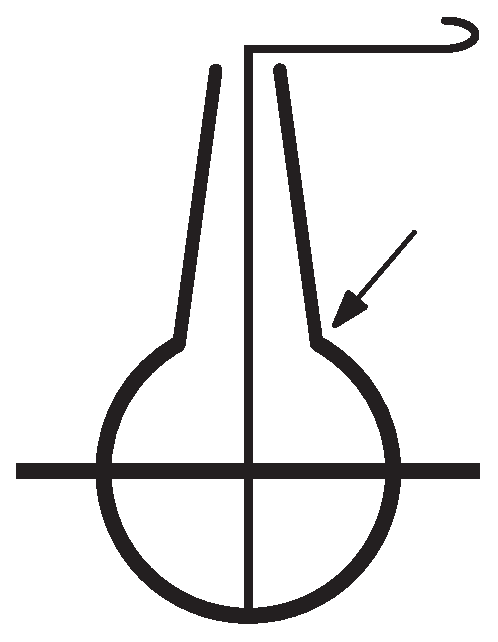
\includegraphics[scale=0.17]{waist.eps}
\circled{2} Berühren des Vibrators \textbf{an der Taille} der Maultrommel \\

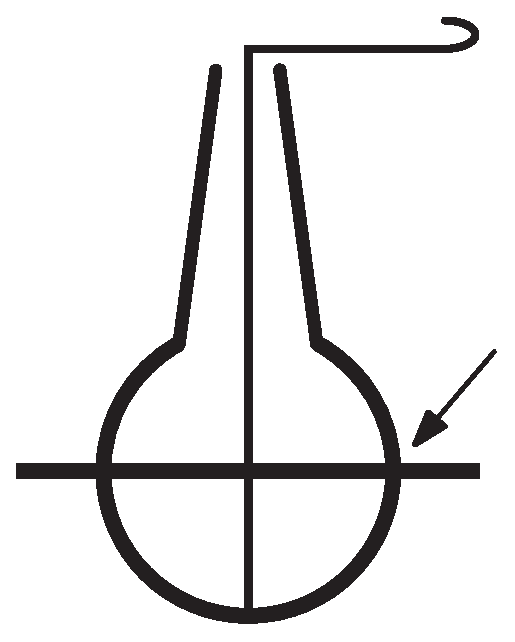
\includegraphics[scale=0.17]{string.eps}
\circled{3} Gleichzeitiges berühren des Vibrators \textbf{an der Basis der Maultrommel und der Saite} \\

Wird beim Spielen in \textbf{Position 1} ein höherer Druck ausgeübt, können durch die Vibration des Maultrommelfußes gegen den Boden des Klavierinneren \textbf{instabile Tonhöhenkonturen} entstehen. Aus diesem Grund wird diese Position manchmal mit einer ungefähren Kontur versehen, die dem Interpreten versuchen kann. \textbf{\circled{4} Schmuckdraht} wird zwischen die Saiten \textbf{A}, \textbf{E'}, \textbf{B'}, \textbf{D''} und \textbf{Es''} bei ,,molto sul ponticello" gelegt, um diese Saiten streichfähig zu machen. Da die unter ,,\textbf{Werkzeuge}" beschriebenen Styroporkugeln oft auf dem Klavierdeckel gerieben werden, um Reibeklänge zu erzeugen, empfiehlt es sich, den Schmuckdraht mit dunklem Kolophonium zu bestreichen, während er \textbf{über den Klavierdeckel} gehalten wird, damit der Staub auf den Deckel fallen kann. \textbf{\circled{5}} Die tiefsten Saiten bis zum D unter dem mittleren C sollten auf der Rückseite mit einer \textbf{dünnen Kette} direkt über den Saiten und \textbf{mit Druckerpapier} über der Kette abgedeckt werden.
\endgroup

\begingroup
\textbf{Werkzeuge: \circled{1}} Für diese Stück werden folgende Werkzeuge benötigt: \\
\circled{1} \textbf{Ein} Plektrum \\
\circled{2} \textbf{Zwei} Styroporkugeln \\
\circled{3} \textbf{Ein} Hartplastikvibrator \\
\circled{4} \textbf{Eine} Maultrommel \\
\circled{5} \textbf{Fünf} lange Stücke von Schmuckdraht \\
\circled{6} Mindestens \textbf{sechs} kleine Magnete \\
\circled{7}  Dünne Kette, Druckerpapier \\
\endgroup

\begingroup
\textbf{Spieltechniken: \circled{1}} Wenn dem Interpreten angewiesen wird, ,,\textbf{mit der Handfläche}" auf den Stimmwirbelmagneten (oder der ,,\textbf{Magnetgruppe}") zu spielen, sollte er seine Handfläche flach auf die Magnete legen, so dass sie möglichst viele von ihnen berührt, und die Hand schnell zur Seite bewegen, wodurch die Magnete gegen die Stimmwirbel rasseln. \textbf{\circled{2}} Bei der Anweisung, auf der ,,\textbf{Tastaturabdeckung}" zu spielen, sollte der Interpret die Tastaturabdeckung gegen die \textbf{Vorderseite} des Klaviers \textbf{schlagen}, damit perkussieren. \textbf{\circled{3}} Notenköpfe, die durch ein \textbf{Akzentzeichen und eine Haltepedal-Artikulation} ersetzt wurden, weisen auf \textbf{Pedal-Percussion} hin, die entweder nur durch \textbf{schnelles Niederdrücken und Loslassen des Haltepedals} oder durch Halten des Haltepedals, Setzen des Sostenuto-Pedals und anschließende Ausführung der einfacheren Pedal-Percussion ausgeführt werden kann, um jede Saite des Klaviers zum Klingen zu bringen. Dem Interpreten muss sich nicht darum kümmern, wie sich diese Pedalvorbereitung auf die Resonanz des gleichzeitigen Tastenspiels auswirkt.
\endgroup

\end{document}